\documentclass{article}
\usepackage{tikz}
\usetikzlibrary{graphs, graphs.standard, quotes}

\begin{document}

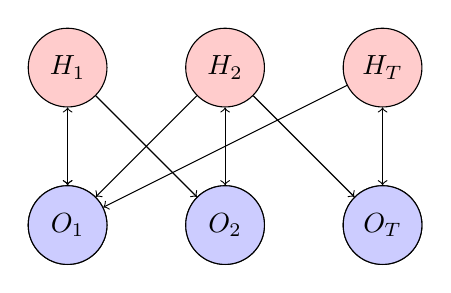
\begin{tikzpicture}[node distance=2cm]
    \tikzset{
        vertex/.style={circle, draw, fill=blue!20, minimum size=1cm},
        hidden/.style={circle, draw, fill=red!20, minimum size=1cm},
    }

    % Nodes
    \node[vertex] (X1) {$X_1$};
    \node[vertex] (X2) [right of=X1] {$X_2$};
    \node[vertex] (XT) [right of=X2] {$X_T$};

    \node[hidden] (H1) [above of=X1] {$H_1$};
    \node[hidden] (H2) [above of=X2] {$H_2$};
    \node[hidden] (HT) [above of=XT] {$H_T$};

    \node[vertex] (O1) [below of=H1] {$O_1$};
    \node[vertex] (O2) [below of=H2] {$O_2$};
    \node[vertex] (OT) [below of=HT] {$O_T$};

    % Edges
    \draw[->] (X1) -- (H1);
    \draw[->] (X2) -- (H2);
    \draw[->] (XT) -- (HT);

    \draw[->] (H1) -- (O1);
    \draw[->] (H2) -- (O2);
    \draw[->] (HT) -- (OT);

    \draw[->] (H1) -- (O2);
    \draw[->] (H2) -- (OT);

    \draw[->] (H1) -- (O1);
    \draw[->] (H2) -- (O1);
    \draw[->] (HT) -- (O1);
\end{tikzpicture}

\end{document}